\documentclass{article}
\usepackage[utf8]{inputenc}
\usepackage{hyperref}

\usepackage{graphicx}
\graphicspath{ {./images/} }
\usepackage{wrapfig}

\usepackage[backend=biber,
bibencoding=ascii,
style=mla,
citestyle=numeric,
sorting=ynt
]{biblatex}
\addbibresource{bibliography.bib}


\title{Collaborative Learning: \\
\normalsize Strategies and Platform Development
}
\author{Paul Baier}
\date{April 20, 2020}

\begin{document}

\maketitle

\begin{abstract}
Throughout the past few years there has been a growing interest among educators to use tools to enhance the student learning experience, sometimes referred to as "Learning Objects" (LO) or "Information and Communication Technology (ICT). As a result, more recent research has been directed to the creation of student-centered educational platforms. The goal of this project is to design and develop a highly extensible, open source, game-based webapp. The platform can be used by instructors to create custom and programmable assessment activities and researchers to explore the effects of different hypotheses involving student collaboration in a classroom setting. Depending on an interplay of factors such as class size, the nature of the material, and personal preferences, instructors may have different ideas and notions of what the ideal student collaboration activity should be. In order to cater to the different instructors’ needs, this system gives instructors the ability to control the flow of information between students for a given activity, and allows instructors to define the structure and rules of how a particular activity should be undertaken.
\end{abstract}

\section{Introduction}
A student response system (SRS) is one used in classrooms to get student feedback. There are many SRS games, which we refer to as student response games (SRG).

\section{Literature Review}
In order to identify prior work in the area of educational games we looked at roughly 2000 proceedings from the Frontiers in Education (FIE) conference from 2015-2019. We started our search with the word "kahoot" because our platform's functional design is based off of Kahoot. Within the search results we identified other platforms mentioned that were similar to Kahoot (and therefore also similar to our platform) and recursively searched for those other platforms as well within the proceedings. This search method allowed us to determine other popular platforms researchers were testing that are comparable to Kahoot as well as other SRS/SRG platforms in development. Our search revealed some of the most popular and relevant SRGs currently in production in addition to Kahoot are Socrative\cite{socrative}, Quizizz\cite{quizizz}, and Quizlet\cite{quizlet}. There were also two platforms in development by researchers called Quipid\cite{quipid} and Dysgu\cite{dysgu}.

Of the existing platforms Quizizz most resembles Kahoot and has many customizable features. The main difference between it and Kahoot or our platform is that students move through the quiz at their own pace (limited by the time assigned to each question). To get started a teacher can either choose a preexisting quiz from a library of quizzes organized by topic or they can create their own. If they choose a pre-made quiz, they can use it as is or copy and edit it to their liking. If they choose to create a new quiz, they can search through existing quizzes for questions in addition to creating their own. Question types include multiple choice, checkbox (select all the correct answers), fill-in-the-blank, polls, and open-ended (the last two are ungraded but marked as correct in reports). For each question the teacher can specify the amount of time the student has to answer. Scores for answering a question correctly are determined in part by the time it took the student to answer relative to the time length of the question.  

Socrative is a web application focused on student engagement and tracking. It offers a number of features outside of the scope of our application, however one of its activities, called "Space Race", is comparable.
\begin{wrapfigure}{l}{0.5\textwidth}
    \centering
    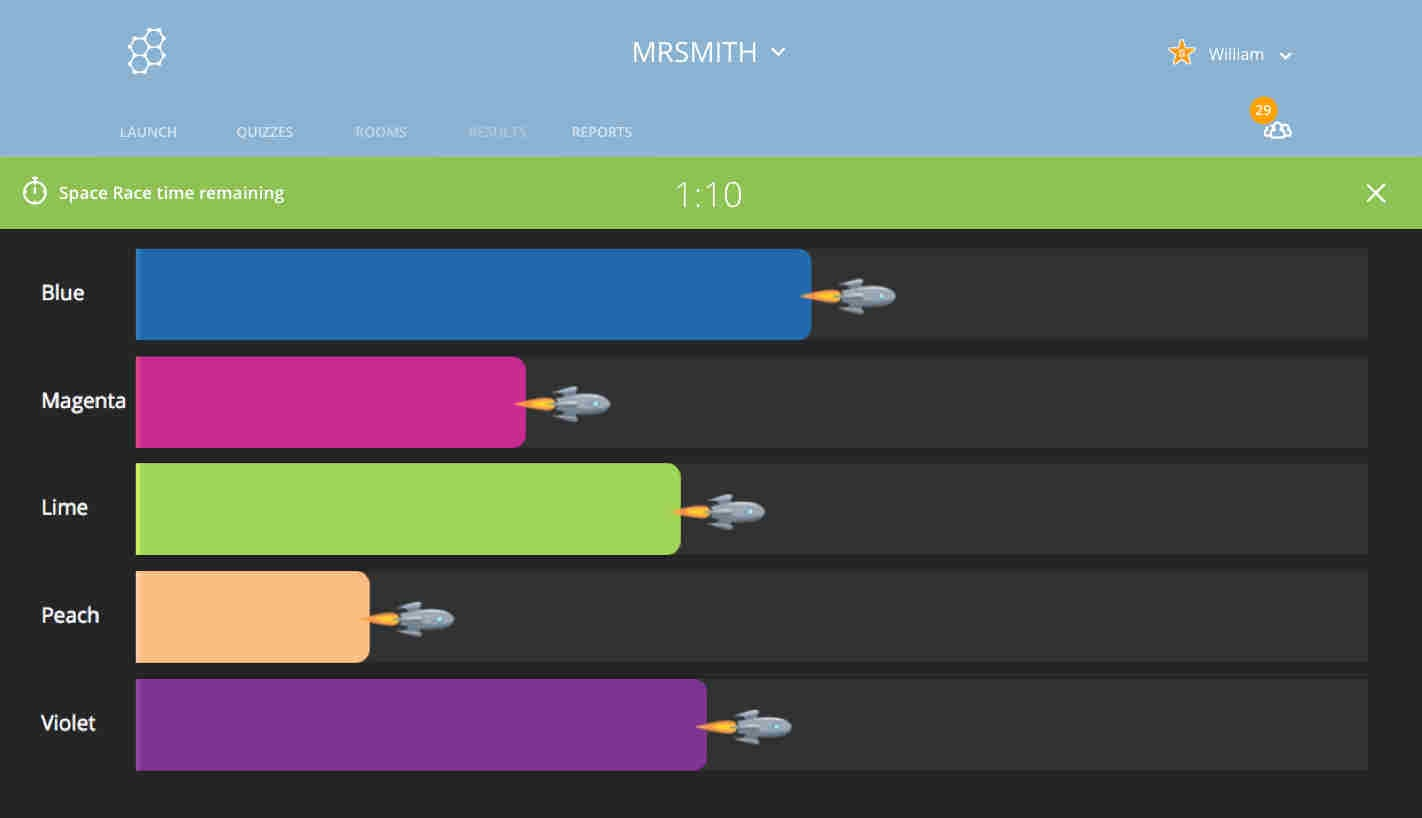
\includegraphics[width=0.5\textwidth]{socrative-space_race}
    \caption{Socrative Space Race \cite{socrative}}
    \label{fig:socrative-space-race}
\end{wrapfigure}
Space Race is a quiz-like game where students are asked a series of questions prearranged by the teacher. Their progress is tracked by little rocket ships (or other icons) that move across the teacher's dashboard when a question is answered correctly (figure \ref{fig:socrative-space-race}). The goal is to be the first individual or team to have their rocket reach across the screen.

Quizzes can be made of multiple choice, true/false, and short answer questions. Other quiz options include the number of teams, how the players are assigned to teams (auto-assigned or student's choice), if the quiz is timed, shuffle the questions, shuffle the answers, show question feedback, show the final score, and if questions can only be attempted once.




Lorem ipsum dolor sit amet, consectetur adipiscing elit, sed do eiusmod tempor incididunt ut labore et dolore magna aliqua. Ut enim ad minim veniam, quis nostrud exercitation ullamco laboris nisi ut aliquip ex ea commodo consequat. Duis aute irure dolor in reprehenderit in voluptate velit esse cillum dolore eu fugiat nulla pariatur. Excepteur sint occaecat cupidatat non proident, sunt in culpa qui officia deserunt mollit anim id est laborum.

Lorem ipsum dolor sit amet, consectetur adipiscing elit, sed do eiusmod tempor incididunt ut labore et dolore magna aliqua. Ut enim ad minim veniam, quis nostrud exercitation ullamco laboris nisi ut aliquip ex ea commodo consequat. Duis aute irure dolor in reprehenderit in voluptate velit esse cillum dolore eu fugiat nulla pariatur. Excepteur sint occaecat cupidatat non proident, sunt in culpa qui officia deserunt mollit anim id est laborum.

\section{Design}
	\subsection{Languages}
		\subsubsection{Python}
		\subsubsection{Django}
\section{Development}
\section{Features}
\section{Future Work}

\printbibliography[title={Bibliography}]


\end{document}

